\section{Запросы базы данных}
\label{sec:database_queries}

Реализация базы данных, её интерфейса и языка запросов --- слишком амбициозный 
проект для данной книги и для знаний читателя в Objective CAML на данный момент. 
Тем не менее, ограничив задачу и используя лучшие возможности функционального 
программирования, можно реализовать достаточно интересное средство для обработки 
запросов. Мы изучим как использовать итераторы и частичное применение для 
написания и выполнения запросов. Также, мы увидим использование типа данных 
инкапсулирующих функциональные значения.

В этом примере мы будем работать над базой данных содержащей информацию о членах 
ассоциации. База храниться в файле \code{association.dat}.

\subsection{Формат данных}
\label{subsec:data_format}

Для хранения данных, большинство баз данных используют свой собственный, так 
называемый \enq{проприетарный} формат. Чаще всего, есть возможность 
экспортировать эти данные в текстовый формат. Вот одна из возможных структур:

\begin{itemize}
	\item база данных есть набор карточек, разделённых возвратом каретки;

	\item каждая карточка есть набор полей, разделённых определённым 
сепаратором, \code{':'} в данном случае;

	\item поле есть строка, не содержащая ни сепаратор \code{':'}, ни возврат 
каретки;

	\item первая карточка есть имена полей, разделённые символом \code{'|'}.
\end{itemize}

Файл ассоциации начинается так:

\begin{lstlisting}[language=OCaml]
Num|Nom|Prenom|Adresse|Tel|Email|Pref|Date|Montant
0:Chailloux:Emmanuel:Université P6:0144274427:ec@lip6.fr:mail:25.12.1998:100.00
1:Manoury:Pascal:Laboratoire PPS::pm@lip6.fr:adr:03.03.1997:150.00
2:Pagano:Bruno:Cristal:0139633963::adr:25.12.1998:150.00
3:Baro:Sylvain::0144274427:baro@pps.fr:mail:01.03.1999:50.00
\end{lstlisting}

\begin{itemize}
	\item \code{Num} номер члена ассоциации

	\item \code{Nom}, \code{Prenom}, \code{Adresse}, \code{Tel} и 
\code{Email} говорят сами за себя
	
	\item \code{Pref} указывает как член предпочитает получать информацию: по 
почте (mail), по емайлу (\code{email}) или по телефону (\code{tel}).
	
	\item \code{Date} и \code{Montant} соответственно дата и сумма последнего 
взноса.
\end{itemize}

Теперь необходимо выбрать формат в котором программа будет хранить данные базы. 
У нас есть выбор: список или вектор карточек. Списком легче манипулировать; 
добавление и удаление карточек являются простыми операциями. Зато векторы 
предоставляют одинаковое время доступа к любой карточке. Так как мы желаем 
использовать все карточки, а не какие-то конкретно, каждый запрос обрабатывает 
все множество карточек. По этой причине мы выбираем списки. Для карточек у нас 
тот же самый выбор: список или вектор строк? В этом случае ситуация обратная; с 
одной стороны формат карточки зафиксирован для всей базы данных и мы не можем 
добавить новые поля. С другой стороны, в зависимости от будущих операции, мы 
используем лишь некоторые поля карточек, соответственно необходимо быстро 
получить к ним доступ.

Вполне естественным решением данной задачи будет использование вектора 
проиндексированного именами полей. Однако подобный тип не возможен в Objective 
CAML, мы воспользуемся обычным вектором (проиндексированный целыми числами) и 
функцией, которая возвращает имя поля в зависимости от индекса.

\begin{lstlisting}[language=OCaml]
# type data_card = string array ;;
# type data_base = { card_index : string -> int ; data : data_card list } ;;
\end{lstlisting}

Реализуем доступ к полю по имени n карточки \code{dc} базы данных \code{db} при 
помощи следующей функции:

\begin{lstlisting}[language=OCaml]
# let field db n (dc:data_card) = dc.(db.card_index n) ;;
val field : data_base -> string -> data_card -> string = <fun>
\end{lstlisting}

Мы принудительно привели тип переменной \code{dc} к \code{data\_card}, тем 
самым наша функция \code{field} принимает лишь вектор строк, а не какой попало.

Проиллюстрируем на небольшом примере.

\begin{lstlisting}[language=OCaml]
# let base_ex = 
   { data = [ [|"Chailloux"; "Emmanuel"|] ; [|"Manoury";"Pascal"|] ]  ;
     card_index = function "Nom"->0 | "Prenom"->1 | _->raise Not_found  } ;;
val base_ex : data_base =
  {card_index=<fun>;
   data=[[|"Chailloux"; "Emmanuel"|]; [|"Manoury"; "Pascal"|]]}
# List.map (field base_ex "Nom") base_ex.data ;;
- : string list = ["Chailloux"; "Manoury"]
\end{lstlisting}

Выражение \code{field base\_ex "Lastname"} вычисляется как функция, которая 
берет на вход карточку и возвращает поле \code{"Lastname"}. Используя 
\code{List.map}, мы применяем эту функцию к каждой карточке базы данных 
\code{base\_ex} и в результате получаем список полей \code{"Lastname"}.

На этом примере показано, как мы собираемся использовать функциональный стиль 
программирования. В данном случае частичное применение функции \code{field} 
определяет функцию доступа к конкретному полю, независимо от числа карточек в 
базе данных. В то же время, в реализации функции \code{field} есть недостаток: 
если мы обращаемся каждый раз к одному и тому же полю, индекс вычисляется 
каждый раз. Мы предпочитаем следующую реализацию.

\begin{lstlisting}[language=OCaml]
# let field base name = 
   let i = base.card_index name in fun (card:data_card) -> card.(i) ;;
val field : data_base -> string -> data_card -> string = <fun>
\end{lstlisting}

Здесь, после применения функции к аргументу, вычисляется индекс поля и 
используется в последующих вычислениях.

\subsection{Чтение базы из файла}
\label{subsec:reading_a_database_from_a_file}

Для Objective CAML, файл с базой данных это множество линий. Наша задача состоит 
в том чтобы прочитать каждую линию, как строку, затем в разбить ее на части при 
помощи сепараторов и таким образом извлечь данные, а также данные для функции 
индексации полей.

\subsubsection{Утилита для обработки линий}

Нам нужна функция \code{split}, которая будет разбивать строку в соответствии с 
определённым разделителем. Для этого мы воспользуемся функцией \code{suffix}, 
возвращающая суффикс строки \code{s} начиная с позиции \code{i}. В этом нам 
помогут три предопределённые функции:

\begin{itemize}
	\item \code{String.length} возвращает длину строки;

	\item \code{String.sub} возвращает подстроку строки s начиная с позиции 
\code{i} и длинной \code{l};

	\item \code{String.index\_from} для строки \code{s} вычисляет начиная с 
позиции \code{n}, позицию первого встреченного символа \code{c}.
\end{itemize}

\begin{lstlisting}[language=OCaml]
# let suffix s i = try String.sub s i ((String.length s)-i) 
                  with Invalid_argument("String.sub") -> "" ;;
val suffix : string -> int -> string = <fun>
# let split c s = 
   let rec split_from n = 
     try  let p = String.index_from s n c 
          in (String.sub s n (p-n)) :: (split_from (p+1)) 
     with Not_found -> [ suffix s n ] 
   in if s="" then [] else split_from 0 ;;
val split : char -> string -> string list = <fun>
\end{lstlisting}

Обратите внимание на обработку исключений в этой функции, в особенности 
исключение \code{Not\_found}.

\subsubsection{Вычисление структуры \code{data\_base}}

Для того чтобы получить из списка вектор, достаточно воспользоваться функцией 
\code{of\_list} из модуля \code{Array}. Вычисление функции индекса из списка 
имени полей может показаться сложной задачей, но к счастью модуль \code{List} 
предоставляет нам все необходимые для этого средства.

У нас имеется список строк, значит нам нужна функция, которая ассоциирует строке 
индекс, то есть её положение или номер в списке.

\begin{lstlisting}[language=OCaml]
# let mk_index list_names = 
   let rec make_enum a b = if a > b then [] else a::(make_enum (a+1) b) in 
   let list_index =  (make_enum 0 ((List.length list_names) - 1)) in 
   let assoc_index_name = List.combine list_names list_index  in 
     function name -> List.assoc name assoc_index_name  ;;
val mk_index : 'a list -> 'a -> int = <fun>
\end{lstlisting}

Для реализации этой функции, мы создаём список индексов, который мы комбинируем 
со списком имён полей. Таким образом вы получаем новый список ассоциаций с 
типом \type{string * int list}. Для того, чтобы найти индекс связанный с 
именем, воспользуемся специально созданной на подобный случай функцией 
\code{assoc} из библиотеки \code{List}. Функция \code{mk\_index} возвращает 
функцию которая берет на входе имя и вызывает \code{assoc} с этим именем и 
списком построенным ранее.

Теперь мы готовы, к тому чтобы написать функцию читающую файлы базы данных в 
указанном формате.

\begin{lstlisting}[language=OCaml]
# let read_base name_file =
   let channel = open_in name_file in
   let split_line = split ':' in
   let list_names = split '|' (input_line channel) in
   let rec read_file () = 
     try 
       let data = Array.of_list (split_line (input_line channel )) in
         data :: (read_file ())
     with End_of_file ->  close_in channel ; []
   in 
     { card_index = mk_index list_names ; data = read_file () } ;;
val read_base : string -> data_base = <fun>
\end{lstlisting}

Считывание записей из файл осуществляется функцией \code{read\_file}, которая 
рекурсивно оперирует входным каналом. Конец файла оповещается исключением 
\code{End\_of\_file}. В этом случае мы закроем канал и вернём пустой список.

Считаем файл ассоциации.

\begin{lstlisting}[language=OCaml]
# let base_ex = read_base "association.dat" ;;
val base_ex : data_base =
  {card_index=<fun>;
   data=
    [[|"0"; "Chailloux"; "Emmanuel"; "Universit\233 P6"; "0144274427";
       "ec@lip6.fr"; "mail"; "25.12.1998"; "100.00"|];
     [|"1"; "Manoury"; "Pascal"; "Laboratoire PPS"; ...|]; ...]}
\end{lstlisting}

\subsection{Общие принципы работы с базой данных}
\label{subsec:general_principles_for_database_processing}

Богатство и сложность обработки множества данных базы пропорциональны богатству 
и сложности используемого языка запросов. Так как в данном случае мы решили 
использовать Objective CAML в качестве языка запросов, {\it a priori}
ограничений на выражение запросов нет! Мы так же хотим предоставить несколько 
простых средств манипуляции карточками и их данными. Для получения желанной 
простоты, необходимо ограничить мощь Objective CAML, для этого определим 
несколько целей и принципов обработки.

Цель обработки данных заключается в получении так называемого состояния базы. 
Создание такого состояния базы можно разбить на три этапа:

\begin{itemize}
	\item выборка по какому–нибудь критерию множества карточек

	\item индивидуальная обработка каждой из выбранных карточек

	\item обработка множества данных полученных из этих карточек 
\end{itemize}

Что мы и изобразили на рисунке \ref{fig:processing_a_request}.

\begin{figure}[h]
	\center{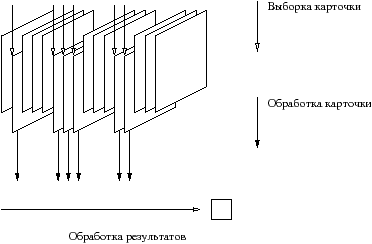
\includegraphics[width=\textwidth] {drafts/book009}}
	\caption{\label{fig:processing_a_request}Обработка запроса}
\end{figure}

В соответствии с этим, нам нужно 3 функции следующих типов:

\begin{itemize}
	\item \type{(data\_card -> bool) -> data\_card list -> data\_card list}
	
	\item \type{(data\_card -> 'a) -> data\_card list -> 'a list}
	
	\item \type{('a -> 'b -> 'b) -> 'a list -> 'b -> 'b}
\end{itemize}

Objective CAML предоставляет три функции высшего порядка, известные как 
итераторы, представленные на странице \ref{??}. Они соответствуют нашей 
спецификации.

\begin{lstlisting}[language=OCaml]
# List.find_all ;;
- : ('a -> bool) -> 'a list -> 'a list = <fun>
# List.map ;;
- : ('a -> 'b) -> 'a list -> 'b list = <fun>
# List.fold_right ;;
- : ('a -> 'b -> 'b) -> 'a list -> 'b -> 'b = <fun>
\end{lstlisting}

После того как мы определим функциональные аргументы, мы сможем воспользоваться 
этими функциями для реализации состояния в три этапа.

Для некоторых запросов нам понадобится следующая функция.

\begin{lstlisting}[language=OCaml]
# List.iter ;;
- : ('a -> unit) -> 'a list -> unit = <fun>
\end{lstlisting}

В случае, когда обработка данных ограничивается выводом на экран, вычислять 
нечего.

В следующих параграфах, мы увидим несколько простых методов обработки данных, а 
так же определение функций выражающих критерии выборки. Небольшой пример в 
заключении этой главы использует эти функции в соответствии с приведёнными выше 
принципами.

\subsection{Критерии выборки}
\label{subsec:selection_criteria}

В конкретном случае, логическая функция, которая определяет критерии выборки 
карточки, есть логическая комбинация свойств данных всех или части полей 
карточки. Каждое поле карточки, представленное строкой, может нести в себе 
информацию другого типа: целое число, число с плавающей запятой, и т.д..

\subsubsection{Критерии выборки по одному полю}

Выборка определённого поля по конкретному критерию будет осуществляется при 
помощи следующей функции \type{data\_base -> 'a -> string -> data\_card -> 
bool}. Параметр типом 'a соответствует типу информации хранимой в поле. Имя 
этого поля указанно аргументом с типом \type{string}.

\paragraph{Поля со строковым типом данных}

Определим два простых теста для работы с этим типом данных: тест на равенство с 
другой строкой и тест на \enq{не пустоту} строки.

\begin{lstlisting}[language=OCaml]
# let eq_sfield db s n dc =  (s = (field db n dc)) ;;
val eq_sfield : data_base -> string -> string -> data_card -> bool = <fun>
# let nonempty_sfield db n dc = ("" <> (field db n dc)) ;;
val nonempty_sfield : data_base -> string -> data_card -> bool = <fun>
\end{lstlisting}

\paragraph{Поля со типом данных число с плавающей запятой}

Для проверки информации содержащей числа с плавающей запятой достаточно 
перевести значение строки содержащей десятичное число в тип \type{float}. Вот 
несколько примеров полученных использованием настраиваемой функции 
\code{tst\_ffield}:

\begin{lstlisting}[language=OCaml]
# let tst_ffield r db v n dc = r v (float_of_string (field db n dc)) ;;
val tst_ffield :
  ('a -> float -> 'b) -> data_base -> 'a -> string -> data_card -> 'b = <fun>
# let eq_ffield = tst_ffield (=) ;;  
# let lt_ffield = tst_ffield (<) ;;  
# let le_ffield = tst_ffield (<=) ;; 
(* etc. *) 
\end{lstlisting}

Тип у данных функций:

\type{data\_base -> float -> string -> data\_card -> bool}.

Этот тип информации немного сложней, он зависит от представления даты в базе 
данных и требует определения способа сравнения дат.

Установим формат даты карточки как строку \code{дд.мм.гггг}. Для того чтобы 
получить дополнительные возможности сравнения, добавим в формат даты символ 
\code{'\_'}, заменяющий день, месяц или год. Даты сравниваются в 
лексикографическом порядке в формате \type{(год, месяц, день)}. Для того чтобы 
мы могли пользоваться выражениями как \enq{до июля 1998}, будем использовать 
сопоставление с образцом даты: \enq{\_.07.1998}. Сравнение даты с образцом 
реализуется функцией \code{tst\_dfield}, которая анализирует образец и создаёт 
{\it ad hoc} сравнивающую функцию. Для того чтобы определить эту универсальную 
функцию проверки даты, нам понадобятся несколько дополнительных функций.

Напишем две функции преобразующие дату (\code{ints\_of\_string}) и образцы даты 
(\code{ints\_of\_dpat}) в триплет целых чисел. Мы заменим символ \code{'\_'} 
образца на целое число 0.

\begin{lstlisting}[language=OCaml]
# let split_date = split '.' ;;
val split_date : string -> string list = <fun>
# let ints_of_string d =
   try  match split_date d with
           [j;m;a] -> [int_of_string a; int_of_string m; int_of_string j]
          |    _   -> failwith "Bad date format"
   with Failure("int_of_string") -> failwith "Bad date format" ;;
val ints_of_string : string -> int list = <fun>

# let ints_of_dpat d =
   let int_of_stringpat = function "_" -> 0 | s -> int_of_string s
   in try  match split_date d with
               [j;m;a] -> [ int_of_stringpat a; int_of_stringpat m; 
                            int_of_stringpat j ]
             | _ -> failwith "Bad date format"
      with Failure("int_of_string") -> failwith "Bad date pattern" ;;
val ints_of_dpat : string -> int list = <fun>
\end{lstlisting}

Напишем функцию теста, которая использует отношение целых \code{r}. Здесь мы 
реализуем лексикографический порядок, при этом мы обрабатываем специальный 
случай с нулём.

\begin{lstlisting}[language=OCaml]
# let rec app_dtst r d1 d2 = match d1, d2 with
    [] , [] -> false
  | (0::d1) , (_::d2) -> app_dtst r d1 d2
  | (n1::d1) , (n2::d2) -> (r n1 n2) || ((n1 = n2) && (app_dtst r d1 d2))
  | _, _ -> failwith "Bad date pattern or format" ;;
val app_dtst : (int -> int -> bool) -> int list -> int list -> bool = <fun>
\end{lstlisting}

Наконец, определим универсальную функцию \code{tst\_dfield} со следующими 
аргументами: отношение \code{r}, база данных \code{db}, образец \code{dp}, имя 
поля \code{nm} и карточка \code{dc}. Эта функция проверяет, что образец и 
извлечённое поле удовлетворяют отношение.

\begin{lstlisting}[language=OCaml]
# let tst_dfield r db dp nm dc = 
  r (ints_of_dpat dp) (ints_of_string (field db nm dc)) ;;
val tst_dfield :
  (int list -> int list -> 'a) ->
  data_base -> string -> string -> data_card -> 'a = <fun>
\end{lstlisting}

Теперь применим функцию к трём отношениям.

\begin{lstlisting}[language=OCaml]
# let eq_dfield = tst_dfield (=) ;;
# let le_dfield = tst_dfield (<=) ;;
# let ge_dfield = tst_dfield (>=) ;;
\end{lstlisting}

Тип этих функций следующий:

\type{data\_base -> string -> string -> data\_card -> bool}.

\subsubsection{Композиция критериев}

Три первые аргумента проверок, которые мы определили --- база данных, значение 
и имя поля. Когда мы пишем запросы базы данных, значения этих аргументов 
известны. Для базы \code{base\_ex} проверка \enq{до июля 1998} пишется 
следующим образом.

\begin{lstlisting}[language=OCaml]
# ge_dfield base_ex "_.07.1998" "Date" ;;
- : data_card -> bool = <fun>
\end{lstlisting}

Получается, что проверка это функция имеющая тип \type{data\_card -> bool}. 
Теперь нам нужно получить логические комбинации результатов подобных функций, 
применённых к одной и той же карточке. Для этого воспользуемся следующим 
итератором.

\begin{lstlisting}[language=OCaml]
# let fold_funs b c fs dc =
  List.fold_right (fun f -> fun r -> c (f dc) r) fs b ;;
val fold_funs : 'a -> ('b -> 'a -> 'a) -> ('c -> 'b) list -> 'c -> 'a = <fun>
\end{lstlisting}

Здесь \code{b} --- значение базы, функция \code{c} --- логический оператор, 
\code{fs} --- список функций проверки по полю и \code{dc} --- карточка.

В следующем примере получаем конъюнкцию (логическое произведение) и дизъюнкцию 
(логическая сумма) списка проверок.

\begin{lstlisting}[language=OCaml]
# let and_fold fs = fold_funs true (&) fs ;;
val and_fold : ('a -> bool) list -> 'a -> bool = <fun>
# let or_fold fs = fold_funs false (or) fs ;;
val or_fold : ('a -> bool) list -> 'a -> bool = <fun>
\end{lstlisting}

Для удобства определим отрицание функции проверки.

\begin{lstlisting}[language=OCaml]
# let not_fun f dc = not (f dc) ;;
val not_fun : ('a -> bool) -> 'a -> bool = <fun>
\end{lstlisting}

Для того, чтобы выбрать карточку, дата которой находится в определённом 
интервале, воспользуемся комбинаторными операторами.

\begin{lstlisting}[language=OCaml]
# let date_interval db d1 d2 = 
  and_fold [(le_dfield db d1 "Date"); (ge_dfield db d2 "Date")] ;;
val date_interval : data_base -> string -> string -> data_card -> bool =
  <fun>
\end{lstlisting}

\subsection{Обработка и вычисление}
\label{subsec:processing_and_computation}

Трудно представить себе все возможные обработки карточек или множество данных 
полученных после этой обработки. Тем не менее можно с уверенностью определить 
два класса таких обработок: численное вычисление и форматирование данных для 
печати. Рассмотрим каждый каждый случай на примере.

\subsubsection{Форматирование}

Подготовим к печати строку, содержащую имя члена ассоциации и кое-какую 
информацию.

Начнём с определения функции, которая из списка строк и разделителя создаёт 
строку состоящую из элемент списка разделённых сепаратором.

\begin{lstlisting}[language=OCaml]
# let format_list c = 
  let s = String.make 1 c in  
  List.fold_left (fun x y -> if x="" then y else x^s^y) "" ;;
val format_list : char -> string list -> string = <fun>
\end{lstlisting}

Определим функцию \code{extract}, которая создаёт список из полей с 
информацией, она извлекает из каждой карточки данные полей, имена которых 
переданы в списке.

\begin{lstlisting}[language=OCaml]
# let extract db ns dc = 
   List.map (fun n -> field db n dc) ns  ;;
val extract : data_base -> string list -> data_card -> string list = <fun>
\end{lstlisting}

Функция форматирования для печати выглядит следующим образом.

\begin{lstlisting}[language=OCaml]
# let format_line db ns dc =
  (String.uppercase (field db "Nom" dc))
  ^" "^(field db "Prenom" dc)
  ^"\t"^(format_list '\t' (extract db ns dc))
  ^"\n" ;;
val format_line : data_base -> string list -> data_card -> string = <fun>
\end{lstlisting}

Аргумент \code{ns} является списком с именами полей, которые нас интересуют. 
Поля разделены символом табуляции (\code{'\\t'}), а строка заканчивается 
возвратом каретки.

Вот как можно вывести на экран имена и фамилии членов ассоциации.

\begin{lstlisting}[language=OCaml]
# List.iter print_string (List.map (format_line base_ex []) base_ex.data) ;;
CHAILLOUX Emmanuel	
MANOURY Pascal	
PAGANO Bruno	
BARO Sylvain	
- : unit = ()
\end{lstlisting}

\subsubsection{Числовое вычисление}

Давайте вычислим сумму членских взносов для определённого множества карточек. 
Для этого достаточно извлечь нужное поле, привести к целому типу и вычислить 
сумму. Нужный результат может быть получен композицией этих функций. Для 
упрощения записи, определим инфиксный оператор композиции.

\begin{lstlisting}[language=OCaml]
# let (++) f g x = g (f x) ;;
val ++ : ('a -> 'b) -> ('b -> 'c) -> 'a -> 'c = <fun>
\end{lstlisting}

Воспользуемся этим оператором в следующем определении.

\begin{lstlisting}[language=OCaml]
# let total db dcs =
   List.fold_right ((field db "Montant") ++ float_of_string ++ (+.)) dcs 0.0 ;;
val total : data_base -> data_card list -> float = <fun>
\end{lstlisting}

Аналогичным образом можно применить эту функцию ко всей базе денных.

\begin{lstlisting}[language=OCaml]
# total base_ex base_ex.data ;;
- : float = 450
\end{lstlisting}

\subsection{Пример}
\label{subsec:an_example}

В заключении, проиллюстрируем на примере принципы, которые мы представили ранее 
в этой главе.

Рассмотрим два типа запроса базы данных:

\begin{itemize}
	\item запрос, возвращающий два списка, каждый из них содержит имя члена 
ассоциации, а так же электронный адрес для первого списка и почтовый адрес для 
второго, в зависимости от предпочтений.

	\item запрос, возвращающий состояние взносов на указанный период времени. 
Это  состояние будет хранить имена, фамилии, дату, взнос и сумму всех взносов.
\end{itemize}

\subsubsection{Списки адресов}

Для создания этих списков мы сначала выбираем в соответствии со значением поля 
\code{"Pref"} релевантные карточки, затем используем функцию 
\code{format\_line}.

\begin{lstlisting}[language=OCaml]
# let adresses_postales db =
  let dcs = List.find_all (eq_sfield db "adr" "Pref") db.data in
   List.map (format_line db ["Adresse"]) dcs ;;
val adresses_postales : data_base -> string list = <fun>

# let adresses_electroniques db =
  let dcs = List.find_all (eq_sfield db "mail" "Pref") db.data in
   List.map (format_line db ["Email"]) dcs ;;
val adresses_electroniques : data_base -> string list = <fun>
\end{lstlisting}

\subsubsection{Состояние взносов}

Вычисление состояния взносов выполняется по обычному принципы: выборка, затем 
обработка. В данном случае обработка состоит из двух частей: форматирование и 
вычисление общей суммы взносов.

\begin{lstlisting}[language=OCaml]
# let etat_cotisations db d1 d2 =
  let dcs = List.find_all (date_interval db d1 d2) db.data in
  let ls = List.map (format_line db ["Date";"Montant"]) dcs in
  let t = total db dcs in
   ls, t ;;
val etat_cotisations : data_base -> string -> string -> string list * float =
  <fun>
\end{lstlisting}

В результате этой функции мы получим пару состоящую из списка строк с 
информацией и суммы взносов.

\subsubsection{Основная программа}

Основная программа состоит из интерактивного цикла, выводящего результат 
запроса, который пользователь выбрал из меню. Здесь мы используем императивный 
стиль программирования, за исключением вывода результата при помощи итератора.

\begin{lstlisting}[language=OCaml]
# let main() =
  let db = read_base "association.dat" in
  let fin = ref false in
   while not !fin do
    print_string" 1: liste des adresses postales\n";
    print_string" 2: liste des adresses électroniques\n";
    print_string" 3: cotisations\n";
    print_string"  0 sortie\n";
    print_string"Votre choix : ";
    match read_int() with
      0 -> fin := true
    | 1 -> (List.iter print_string (adresses_postales db))
    | 2 -> (List.iter print_string (adresses_electroniques db))
    | 3
     -> (let d1 = print_string"Date de début : "; read_line() in
         let d2 = print_string"Date de fin : "; read_line() in
         let ls, t = etat_cotisations db d1 d2 in
          List.iter print_string ls;
          print_string"Total : "; print_float t; print_newline())
    | _ -> ()
   done;
   print_string"bye\n" ;;
val main : unit -> unit = <fun>
\end{lstlisting}

Мы вернёмся к этому примеру в главе \ref{??}, чтобы добавить к нему интерфейс 
при помощи web навигатора.

\subsection{Дополнительные возможности}
\label{subsec:further_work}

Вполне естественным будет добавить в базу данных нашего примера информацию о 
типе каждого поля. Эта информация пригодится в случае если мы хотим определить 
универсальные (generic) операторы сравнения со следующим типом \type{data\_base 
-> 'a -> string -> data\_card -> bool}. Имя поля (третий аргумент) позволяет 
передавать управление соответствующей функции сравнения и проверки. 
